\section{Sec.~III: Von Neumann algebras and entanglement: type I and II}

Sec.~II built the whole apparatus — algebras, states, projections, the type classification, and the GNS
construction — but always working with a fixed algebra $\M$ sitting inside some ambient $B(\HH)$, with no
particular state singled out for special attention. This section asks the question the whole framework was
built to answer: given a specific physical state $\ket\Psi$, what does the \emph{type} of $\M$ tell you about
how $\Psi$ entangles the subsystem $\M$ describes with everything outside it? Type I and type II are handled
here, because both still have a trace, so a density operator and an entropy can still be defined by a direct
generalization of the formulas you already know. Type III — where no trace exists at all — needs an entirely
different tool, and is deferred to Sec.~IV.

\begin{figure}[htbp]
\centering
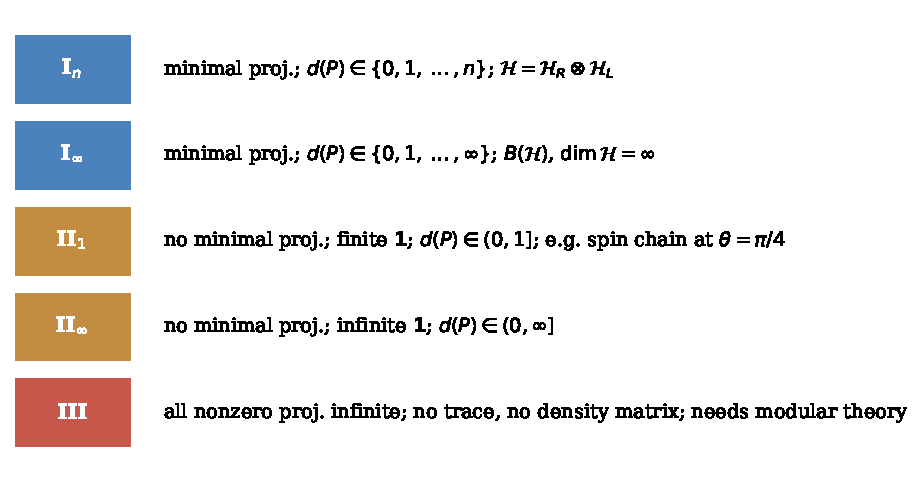
\includegraphics[width=0.88\textwidth]{figs/fig_type_chart.pdf}
\caption{The taxonomy of von Neumann algebra factors: classified by Murray and von Neumann according to the range of their projection dimension function $d(\mathcal{P}(\M))$ and the existence of a tracial state $\tau$. Type I possesses minimal projections (rank-one rays); Type II has no minimal projections but supports a trace (finite for $\mathrm{II}_1$, semifinite for $\mathrm{II}_\infty$); Type III has neither minimal projections nor a trace, exhibiting purely infinite projection dimensions.}
\label{fig:type_chart}
\end{figure}

\begin{table}[htbp]
\centering
\footnotesize
\begin{tabularx}{\textwidth}{@{}l p{2.2cm} l p{2.6cm} X l@{}}
\toprule
\textbf{Factor} & \textbf{Proj. Dim. $d(\mathcal{P})$} & \textbf{Trace $\tau$} & \textbf{Density Matrix $\rho_\M$} & \textbf{Physical System} & \textbf{Entropy Status} \\
\midrule
$\mathrm{I}_n$ & $\{0, 1, \dots, n\}$ & Yes (finite) & $\rho_R = \Tr_L\ket\Psi\bra\Psi$ & $n$-level system / qubits & $S \ge 0$ \\
$\mathrm{I}_\infty$ & $\{0, 1, 2, \dots, \infty\}$ & Yes (semifinite) & Fock space $\rho$ & Harmonic oscillator & Well-defined \\
$\mathrm{II}_1$ & $[0, 1]$ (continuous) & $\tau(\id)=1$ & $\rho_\M \in \M$ & $\infty$ Bell pairs ($\theta=\frac{\pi}{4}$) & $S \le 0$ (vs max-mixed) \\
$\mathrm{II}_\infty$ & $[0, \infty]$ (continuous) & Semifinite & $\rho_\M = e^{-K_\Psi - p}$ & Crossed product $\M \rtimes \mathbb{R}$ & $S_{\rm gen} = \frac{\langle\hat A\rangle}{4G_N} + S_{\rm bulk}$ \\
$\mathrm{III}_0$ & $\{0, \infty\}$ & None & No density matrix & Non-ergodic flows & Ill-defined \\
$\mathrm{III}_\lambda$ & $\{0, \infty\}$ & None & No density matrix & Spin chain ($\tan^2\theta = \lambda$) & Relative $S(\rho\|\sigma)$ only \\
$\mathrm{III}_1$ & $\{0, \infty\}$ & None & No density matrix & QFT subregion / Rindler & Relative only / crossed \\
\bottomrule
\end{tabularx}
\caption{Complete classification of von Neumann algebra factors and their physical, operational, and thermodynamic properties.}
\label{tab:factor_taxonomy}
\end{table}

\subsection{Sec.~III.A: density operators for type I and II algebras}

Here is the key new formula, and it deserves to be read as slowly as the definition of $\M$ itself was.
Suppose the full system is in a state $\ket\Psi\in\HH$, and $\M$ is a von Neumann algebra with a trace $\tr$
(so, by Sec.~II.C, type I or type II). Define $\rho_\M\in\M$ to be the operator satisfying
\[
\tr(A\rho_\M) = \braket{\Psi|A|\Psi} \qquad \text{for every } A\in\M
\]
(eq.~3.1). Positivity of $\tr$ guarantees this equation has a unique solution $\rho_\M$, and that the
resulting $\rho_\M$ is itself positive and correctly normalized — i.e., it genuinely deserves to be called a
density operator (footnote~18 of the paper flags a subtlety worth restating: it matters that $\rho_\M$ is
required to belong to $\M$ itself, not merely to $B(\HH)$ — the equation is being solved \emph{within} the
algebra). With $\rho_\M$ in hand, the entanglement entropy is defined exactly as you'd expect,
\[
S_\M \equiv -\tr(\rho_\M\log\rho_\M)
\]
(eq.~3.2) — formally identical to the ordinary formula $S_R=-\Tr(\rho_R\log\rho_R)$, just with $\tr$ (the
algebra's own, possibly renormalized trace from Sec.~II.C) standing in for the ordinary Hilbert-space trace,
and $\rho_\M$ standing in for the ordinary reduced density matrix.

Stop and compare this to the formula you already know, $\rho_R=\Tr_L\ket\Psi\!\bra\Psi$ (a partial trace).
That formula needs the complement $L$ to be given explicitly, as a separate tensor factor you can sum over —
you need to know about the part of the world you \emph{cannot} access in order to build an object describing
the part you \emph{can}. Equation~3.1 needs nothing of the sort: it's a self-contained equation stated purely
in terms of $\M$'s own trace and expectation values of $\M$'s own operators. This is worth stating as
explicitly as the paper does in its own remark: since you only have access to $\M$, in what sense does
$\rho_\M$, defined this way, capture anything about entanglement with the outside world at all? The paper's
own promise (repeated here, since it's the right way to hold the question while reading the rest of the
section): the answer depends entirely on which \emph{type} $\M$ turns out to be, and working through that
answer, type by type, is the entire content of the rest of Sec.~III and all of Sec.~IV.

\subsection{Sec.~III.B: type I algebras}

\subsubsection*{The type I factor case: nothing is lost}

When $\M$ is a type I \emph{factor}, Sec.~II.C already established $\HH=\HH_R\otimes\HH_L$,
$\M=B(\HH_R)\otimes\id_L$, $\tr=\Tr_{\HH_R}$, $\M'=\id_R\otimes B(\HH_L)$ (eq.~3.3). Plug this into the
right-hand side of eq.~3.1: using the ordinary partial-trace formula, $\braket{\Psi|A|\Psi}=\Tr_{\HH_R}(\rho_R
A)$ for $A\in\M$ (eq.~3.4), where $\rho_R=\Tr_{\HH_L}\ket\Psi\bra\Psi$ is the ordinary reduced density matrix
you already know. Comparing this to the defining equation of $\rho_\M$ (eq.~3.1), and using $\tr=\Tr_{\HH_R}$,
you read off immediately: $\rho_\M=\rho_R$. The new, algebra-intrinsic definition and the old,
partial-trace definition give \emph{exactly} the same operator, whenever a type I factorization is available.
Nothing is lost by switching definitions — you can check this is consistent rather than just asserted, since
both sides of eq.~3.1 are now completely explicit ordinary-linear-algebra objects.

Two remarks the paper makes here are worth keeping, because they're exactly the seeds of everything that
happens once type I stops being available:
\begin{enumerate}
\item The two approaches are conceptually very different, even when they agree numerically. Equation~2.2
needs the full global state $\ket\Psi$, including the part living in $\HH_L$ that you have no access to, in
order to build $\rho_R$. Equation~3.1 needs only expectation values of operators in $\M$ — data an
$R$-observer could, in principle, actually collect. The fact that these two completely different-looking
recipes produce the same answer, in the type I case, is itself the thing worth remembering when type I stops
holding: the entanglement information was, all along, fully recoverable from $\M$'s own internal data; the
tensor-product recipe was just a more roundabout way of getting the same answer, one that happens to break
once no factorization exists.
\item Because $\tr$ (equal here to the ordinary $\Tr_{\HH_R}$) genuinely counts basis states of an honest
Hilbert space $\HH_R$, $S_\M=S_R$ inherits a completely ordinary statistical interpretation — the usual
``number of effectively occupied states'' reading of entropy. This interpretation, too, is about to become
much more delicate once you leave type I.
\end{enumerate}

\subsubsection*{General type I: a nontrivial center, and where lattice gauge theory fits}

If $\M$ is type I but \emph{not} a factor (it has a nontrivial center — recall the block-diagonal
$P_1,P_2$ worked example from Sec.~II.B.2 of this companion), the Hilbert space decomposes into a direct sum
of sectors, one for each value $\alpha$ of the central (classical) label:
\[
\HH=\bigoplus_\alpha\HH_\alpha, \quad \HH_\alpha=\HH_{R\alpha}\otimes\HH_{L\alpha}, \qquad
\M=\bigoplus_\alpha\big(B(\HH_{R\alpha})\otimes\id_{L\alpha}\big)
\]
(eqs.~3.5--3.6) — within each sector, the ordinary tensor-product story holds exactly as in the factor case
above; the different sectors just sit side by side, never mixing (any operator in $\M$ acts block-diagonally,
never sending a state in sector $\alpha$ to a state in a different sector $\alpha'$). The trace is built
sector by sector, $\tr A=\sum_\alpha\Tr_{\HH_{R\alpha}}A_\alpha$ (eq.~3.7), and a general state $\rho$ on
$\HH$ decomposes as $\rho=\bigoplus_\alpha p_\alpha\rho_\alpha$ — a classical probability $p_\alpha$ of being
in sector $\alpha$, times an ordinary (normalized) density matrix $\rho_\alpha$ within that sector (eq.~3.8).
Working through eq.~3.1 sector by sector gives $\rho_\M=\bigoplus_\alpha p_\alpha(\rho_{R\alpha}\otimes
\id_{L\alpha})$ (eq.~3.9, with $\rho_{R\alpha}=\Tr_{\HH_{L\alpha}}\rho_\alpha$ the ordinary reduced density
matrix within sector $\alpha$), and plugging this into eq.~3.2 gives an entropy that cleanly splits into two
recognizable pieces,
\[
S_\M = -\sum_\alpha p_\alpha\log p_\alpha \;+\; \sum_\alpha p_\alpha S_\alpha ,
\qquad S_\alpha=-\tr_\alpha(\rho_{R\alpha}\log\rho_{R\alpha})
\]
(eq.~3.10): an ordinary classical (Shannon) entropy of \emph{which sector you're in}, plus the
probability-weighted average of the ordinary quantum entanglement entropy \emph{within} each sector. Nothing
here is conceptually new — it's exactly what you'd compute by hand if someone told you ``the system is either
in configuration A with probability $p_A$ (itself entangled some amount $S_A$) or configuration B with
probability $p_B$ (entangled some amount $S_B$), and you don't know which'' — but it's worth seeing it fall
directly out of the single unified formula, eq.~3.1, rather than needing to be reasoned out from scratch each
time.

\begin{quote}
\textit{Worked example: superselection sectors and entanglement in a 2-site lattice gauge model.} Consider a spatial lattice with two sites ($x_1, x_2$) connected by a gauge link carrying electric flux $E \in \{0, 1\}$. The physical Hilbert space decomposes into superselection sectors labeled by the central electric flux $q \in \{0, 1\}$ passing across the bipartition cut between the sites:
\[
\HH_{\text{phys}} = \HH_{q=0} \oplus \HH_{q=1} = (\HH_{R,0}\otimes\HH_{L,0}) \oplus (\HH_{R,1}\otimes\HH_{L,1}) .
\]
Suppose a physical state is prepared as a mixture of these sectors:
\[
\rho = p_0\,\rho_0 \oplus p_1\,\rho_1 , \qquad p_0 = 0.8, \quad p_1 = 0.2 ,
\]
where in sector $q=0$ the two sites are maximally entangled Bell pairs with reduced density matrix $\rho_{R,0} = \operatorname{diag}(1/2, 1/2)$ ($S_0 = \log 2 \approx 0.6931$), while in sector $q=1$ the sites are unentangled product states ($S_1 = 0$).
Evaluating the unified algebraic entropy formula (eq.~3.10):
\begin{enumerate}
\item \textbf{Classical Shannon entropy of the gauge flux:}
\[
H(p) = -p_0\log p_0 - p_1\log p_1 = -0.8\log(0.8) - 0.2\log(0.2) \approx 0.1785 + 0.3219 = 0.5004\text{ nats} .
\]
\item \textbf{Average quantum entanglement within sectors:}
\[
\sum_\alpha p_\alpha S_\alpha = 0.8 \times (\log 2) + 0.2 \times 0 = 0.8 \times 0.693147 = 0.5545\text{ nats} .
\]
\item \textbf{Total algebraic entropy:}
\[
S_\M = H(p) + \sum_\alpha p_\alpha S_\alpha \approx 0.5004 + 0.5545 = 1.0549\text{ nats} .
\]
\end{enumerate}
This demonstrates how the algebraic framework captures both classical gauge flux fluctuations and genuine quantum entanglement in a single formula without requiring a spatial tensor factorization.
\end{quote}

This is exactly the situation for the lattice gauge theory example (Ex.~1 from Sec.~I): the algebra of
gauge-invariant local operators is type I (it still has minimal projections, still counts states in the
ordinary way sector by sector) but not a factor (gauge invariance imposes a classical superselection label —
which gauge sector, e.g.\ which total electric flux configuration, you're in). The single formula~3.1 handles
this uniformly, with the factorized case (type I factor) simply being the special case of a trivial center
(only one sector, $p_\alpha=1$ for a single $\alpha$). This is the sense in which the algebraic language,
even at this early, still-mostly-familiar stage, is already doing real unifying work.

\subsection{Sec.~III.C: type II algebras}

This is where something genuinely new happens, and the paper's chosen way to show it is to build a type
$\mathrm{II}_1$ factor completely explicitly, by hand, out of the $N\to\infty$ Bell-pair chain from
Sec.~II.E of this companion. It's worth doing every step of this construction, because it is the first
place in the paper where you can watch an entirely new kind of mathematical object get built in front of you,
out of nothing more exotic than an infinite chain of ordinary qubits.

\subsubsection*{Sec.~III.C.1: building a trace at $\theta=\pi/4$}

Recall the setup from Sec.~II.E: $\M\equiv\M_R$ is the von Neumann algebra of operators acting on the
right-hand spins of the chain, built via GNS from the algebra of finite-energy operations $\Alg_R$ and the
state $\omega_\theta(A)=\braket{\Phi_\theta|A|\Phi_\theta}$. Fix $\theta=\pi/4$ (every pair maximally
entangled) and \emph{define}
\[
\tr A \equiv \braket{\Phi_{\pi/4}|A|\Phi_{\pi/4}} , \qquad A\in\M .
\]
(eq.~3.11.) This looks, on the surface, exactly like an ordinary expectation value — nothing distinguishes it
notationally from $\omega_{\pi/4}(A)$ already defined in Sec.~II.E. The claim being made is that, specifically
at $\theta=\pi/4$, this particular expectation value happens to \emph{also} satisfy the cyclic property
$\tr(AB)=\tr(BA)$ that defines a trace (Sec.~II.B.3) — and it's worth verifying this rather than just
believing it, since it is the single fact the entire rest of this subsection rests on.

\textbf{Step 1: a single pair.} Take one spin pair at $\theta=\pi/4$, in the state $\ket{\phi_{\pi/4}}=
\tfrac1{\sqrt2}(\ket{00}+\ket{11})$, and let $a = \begin{pmatrix} a_{00} & a_{01} \\ a_{10} & a_{11} \end{pmatrix}$ be any operator acting on the right spin alone ($a\otimes\id_L$). Let us compute the expectation value by expanding the state:
\begin{align*}
\braket{\phi_{\pi/4}|a\otimes\id_L|\phi_{\pi/4}} &= \frac{1}{2}\left(\bra{00}+\bra{11}\right)(a\otimes\id_L)\left(\ket{00}+\ket{11}\right) \\
&= \frac{1}{2}\left( \braket{00|a\otimes\id|00} + \braket{00|a\otimes\id|11} + \braket{11|a\otimes\id|00} + \braket{11|a\otimes\id|11} \right) \\
&= \frac{1}{2}\left( a_{00}\braket{0|0}_L + a_{01}\braket{0|1}_L + a_{10}\braket{1|0}_L + a_{11}\braket{1|1}_L \right) \\
&= \frac{1}{2}\left( a_{00} + a_{11} \right) = \frac{1}{2}\Tr_2(a) .
\end{align*}
(eq.~3.12, with $\Tr_2$ the ordinary $2\times2$ matrix trace) — the expectation value in a single maximally
entangled pair, of any operator touching only one side of that pair, is exactly one-half the ordinary trace
of that operator. This specific numerical coefficient, $\tfrac12$, is not an accident of notation; it's
exactly $1/\dim(\HH_2)$ for a single qubit, and it will reappear, tracked explicitly, in eq.~3.18 below.

\textbf{Step 2: many pairs.} A general element of $\M_R$ (recall Sec.~II.E, eq.~2.57) is $A=a_1\otimes
a_2\otimes\cdots$, with only finitely many of the $a_i$ different from the identity — say $a_{i_1},\dots,
a_{i_k}$ are the nontrivial ones. Because $\ket{\Phi_{\pi/4}}$ is a product of independent pairs, and each
pair contributes independently via Step~1,
\[
\braket{\Phi_{\pi/4}|A|\Phi_{\pi/4}} = \frac{1}{2^k}\,\Tr_2(a_{i_1})\cdots\Tr_2(a_{i_k})
\]
(eq.~3.13) — the expectation value in the full infinite chain reduces to a product of ordinary $2\times2$
matrix traces, one factor of $\tfrac12$ for each of the $k$ pairs actually touched.

\textbf{Step 3: cyclicity.} Here is the punchline, and it's genuinely just a one-line consequence of Step~2
once you see it: since $\braket{\Phi_{\pi/4}|A|\Phi_{\pi/4}}$ reduces \emph{entirely} to a product of ordinary
$2\times2$ matrix traces, and the ordinary matrix trace is itself cyclic ($\Tr_2(a_ib_i)=\Tr_2(b_ia_i)$ for
each individual pair, a completely standard fact about matrix traces), the whole product inherits cyclicity:
\[
\braket{\Phi_{\pi/4}|AB|\Phi_{\pi/4}} = \braket{\Phi_{\pi/4}|BA|\Phi_{\pi/4}}
\]
(eq.~3.14). This establishes eq.~3.11 as a genuine trace on $\M$. And this is exactly where $\theta=\pi/4$
earns its special status: Step~1's formula, $\braket{\phi_\theta|a|\phi_\theta}=\tfrac12\Tr_2(a)$, is only
exactly true at $\theta=\pi/4$ — for any other angle, the expectation value picks up $\theta$-dependent
weighting that breaks the exact matching to an ordinary matrix trace, and cyclicity fails. While this is often stated without derivation, we can prove the impossibility of any trace directly and rigorously via macroscopic operator condensation:

\begin{keyresult}[: The No-Trace Theorem for the Asymmetric Spin Chain]
\textbf{Theorem:} Let $\Alg_R = \bigotimes_{k=1}^\infty M_2(\mathbb{C})$ be the quasi-local spin chain algebra, and let $\ket{\Phi_\theta} = \bigotimes_{k=1}^\infty (\cos\theta\ket{00} + \sin\theta\ket{11})_k$ with $\theta \in (0, \pi/4)$. Let $\M_R \equiv \pi_\theta(\Alg_R)'' \subseteq B(\HH_\theta)$ be the GNS von Neumann factor.
Then for any $\theta \ne \pi/4$, \textbf{there exists no nonzero normal tracial state on $\M_R$}. Consequently, $\M_R$ is strictly type III.

\textbf{Proof:}
\begin{enumerate}[leftmargin=*]
\item \textbf{Tracial constraint on Pauli commutators:}
Suppose for contradiction that there exists a normal tracial state $\tau: \M_R \to \mathbb{C}$ with $\tau(\id) = 1$. By definition of a trace, $\tau(AB) = \tau(BA)$ for all $A, B \in \M_R$, which implies that $\tau([A, B]) = 0$ for every commutator.
On any individual spin site $k$, consider the Pauli operators $\sigma_x^{(k)}, \sigma_y^{(k)}, \sigma_z^{(k)} \in \Alg_R \subset \M_R$. From the $\mathfrak{su}(2)$ algebra, $[\sigma_x, \sigma_y] = 2i\sigma_z$, which gives:
\[
\sigma_z^{(k)} = \frac{1}{2i}\big[\sigma_x^{(k)}, \, \sigma_y^{(k)}\big] .
\]
Applying the tracial state $\tau$ directly yields:
\[
\tau\big(\sigma_z^{(k)}\big) = \frac{1}{2i}\tau\big([\sigma_x^{(k)}, \, \sigma_y^{(k)}]\big) = 0 \qquad \text{for all } k \ge 1 .
\]

\item \textbf{Vanishing trace of average magnetization:}
Define the macroscopic block-spin average magnetization over the first $N$ sites:
\[
M_N \equiv \frac{1}{N}\sum_{k=1}^N \sigma_z^{(k)} \in \M_R .
\]
By linearity of $\tau$ and the single-site identity above:
\[
\tau(M_N) = \frac{1}{N}\sum_{k=1}^N \tau\big(\sigma_z^{(k)}\big) = 0 \qquad \text{for all } N \ge 1 .
\]

\item \textbf{Macroscopic condensation in the GNS state:}
Now examine $M_N$ in the physical GNS reference state $\ket{\Omega_\theta} \equiv \ket{\Phi_\theta}$. On each entangled pair:
\[
\braket{\phi_\theta | \sigma_z | \phi_\theta} = \cos^2\theta \braket{0|\sigma_z|0} + \sin^2\theta \braket{1|\sigma_z|1} = \cos^2\theta - \sin^2\theta = \cos(2\theta) .
\]
The expectation value of the average magnetization is therefore:
\[
\braket{\Omega_\theta | M_N | \Omega_\theta} = \frac{1}{N}\sum_{k=1}^N \cos(2\theta) = \cos(2\theta) .
\]
Because the state $\ket{\Phi_\theta}$ is an exact product state across different pairs, spin fluctuations at distinct sites $k \ne j$ are completely uncorrelated:
\[
\Braket{\Omega_\theta \Big| \big(\sigma_z^{(k)} - \cos(2\theta)\big)\big(\sigma_z^{(j)} - \cos(2\theta)\big) \Big| \Omega_\theta} = \delta_{kj}\big(1 - \cos^2(2\theta)\big) = \delta_{kj}\sin^2(2\theta) .
\]
The variance of $M_N$ in the GNS representation is:
\[
\big\| \big(M_N - \cos(2\theta)\id\big)\ket{\Omega_\theta} \big\|^2 = \frac{1}{N^2}\sum_{k=1}^N \sin^2(2\theta) = \frac{\sin^2(2\theta)}{N} \xrightarrow{N\to\infty} 0 .
\]

\item \textbf{Strong operator convergence:}
Since $\ket{\Omega_\theta}$ is cyclic and separating for $\M_R$, and $\|M_N\| \le 1$ is uniformly bounded, the vanishing of the variance implies that $M_N$ converges in the strong operator topology on $\HH_\theta$ to a scalar multiple of the identity:
\[
\mathrm{s\text{-}}\lim_{N\to\infty} M_N = \cos(2\theta)\,\id .
\]

\item \textbf{The contradiction:}
By definition of normality, the state $\tau$ is continuous in the weak (and ultraweak) operator topology. Therefore:
\[
\lim_{N\to\infty} \tau(M_N) = \tau\big(\mathrm{s\text{-}}\lim_{N\to\infty} M_N\big) = \tau\big(\cos(2\theta)\id\big) = \cos(2\theta)\,\tau(\id) = \cos(2\theta) .
\]
Comparing this with the exact algebraic result from Step~2:
\[
0 = \lim_{N\to\infty} \tau(M_N) = \cos(2\theta) .
\]
For any non-maximal entangling angle $\theta \in (0, \pi/4)$, we have $\cos(2\theta) > 0$. The equality $0 = \cos(2\theta) > 0$ is a strict contradiction!

Hence no normal tracial state $\tau$ can exist on $\M_R$ when $\theta \ne \pi/4$. With both type I and type II ruled out by the total absence of a trace, $\M_R$ is unavoidably \textbf{type III}. $\blacksquare$
\end{enumerate}
\end{keyresult}

\subsubsection*{Sec.~III.C.2: no minimal projection, and dimensions that are genuine real numbers}

With a bona fide trace in hand, $\M_R$ (at $\theta=\pi/4$) is at least type I or type II — the question is
which. Consider the family of projections built by fixing some finite subset of the spins to be spin-up,
and leaving the rest untouched:
\[
\id \equiv \id_2\otimes\id_2\otimes\cdots, \qquad
P_1 = \id_2\otimes P_\uparrow\otimes\id_2\otimes\cdots, \qquad
P_2 = P_\uparrow\otimes\id_2\otimes P_\uparrow\otimes\id_2\otimes\cdots,
\]
with $P_\uparrow=\begin{psmallmatrix}1&0\\0&0\end{psmallmatrix}$ the projector onto spin-up on a single qubit
(eq.~3.16) — and, in general, you can build a projection this way by choosing \emph{any} finite subset of the
spins and replacing their identity factor with $P_\uparrow$.

Here is the argument that no minimal projection exists, and it's worth seeing why it's airtight rather than
just plausible: take \emph{any} nonzero projection $P$ of this form, built by fixing some finite set of spins.
No matter how many spins it already fixes, you can always find one more spin, currently left as $\id_2$
inside $P$, and replace that one factor with $P_\uparrow$ too — producing a new projection $\widetilde P$ that
is strictly smaller than $P$ (fixing one additional spin can only shrink the corresponding subspace, never
grow it) and still manifestly nonzero. Since this can be done starting from \emph{any} such $P$, with no
exception, there is no smallest one — no projection built this way can be minimal. So $\M_R$ has finite
projections (as you're about to see) but no minimal ones: by the Sec.~II.C classification, this rules out
type I entirely.

Now compute actual dimensions, using the trace normalized so $d(\id)=\tr(\id)=1$ (eq.~3.17 — automatic, since
$\tr(\id)=\braket{\Phi_{\pi/4}|\id|\Phi_{\pi/4}}=1$ by normalization of the state). Using Step~2's formula
above directly: $P_1$ fixes exactly one spin to $P_\uparrow$ (with $\Tr_2(P_\uparrow)=1$), so
$d(P_1)=\tr(P_1)=\tfrac12\Tr_2(P_\uparrow)=\tfrac12$; $P_2$ fixes two spins, so
$d(P_2)=\tr(P_2)=\tfrac1{2^2}\Tr_2(P_\uparrow)\Tr_2(P_\uparrow)=\tfrac14$ (eq.~3.18) — and in general, a
projection fixing $k$ spins has dimension exactly $2^{-k}$. Check this is completely consistent, not just
plausible: for any finite $k$, $2^{-k}>0$ (never actually zero, however large $k$ is), so every one of these
projections is genuinely nonzero and finite — consistent with there being no minimal one (you can always
halve the dimension again by fixing one more spin, but you never reach zero at any finite step).

This is the moment where something with literally no counterpart in ordinary finite-dimensional linear
algebra appears: by taking superpositions of orthogonal projections built this way (and limits of such
superpositions — infinite sums, made rigorous by the completeness built into the von Neumann algebra
structure), you can construct a projection $P$ with $d(P)$ equal to \emph{any} real number in $(0,1]$, not
just the numbers $2^{-k}$ reachable by the simple fixed-spin construction above. Compare this once more to
ordinary quantum mechanics: there, ``the dimension of a subspace'' is always a whole number, obtained by
literally counting basis vectors — there is no such thing as a subspace of dimension $0.31830989\ldots$ (an
arbitrary real number). Here, $d(P)$ genuinely can be any such number, and this continuous range of possible
dimensions, together with the complete absence of a minimal projection, is precisely the defining signature
of type $\mathrm{II}_1$ (Sec.~II.C): finite projections exist and can be directly compared in size, but there
is no smallest possible ``one unit'' of measurement, only an ever-refinable continuum. So: at $\theta=\pi/4$,
$\M=\M_R$ is a type $\mathrm{II}_1$ factor — the first genuinely new object encountered so far in this
companion, and it was built using nothing beyond ordinary spin-$\tfrac12$ qubits and an infinite chain of
them.

\begin{figure}[htbp]
\centering
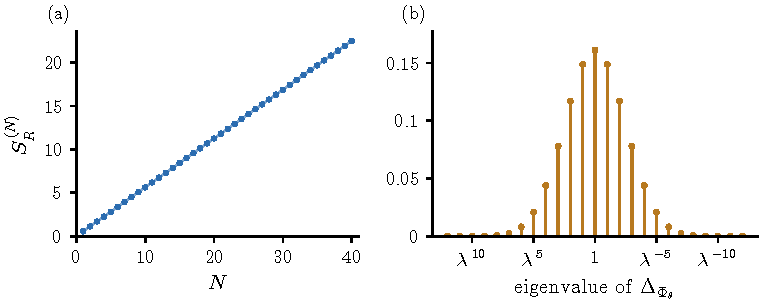
\includegraphics[width=0.78\textwidth]{figs/fig_spin_chain_typeIII.pdf}
\caption{The emergence of non-Type I factor structures from an infinite spin chain: as the number of entangled qubit pairs $N \to \infty$, the discrete eigenvalues of the reduced state merge into a continuous spectrum. At $\theta = \pi/4$, the algebra becomes the hyperfinite Type $\mathrm{II}_1$ factor where projections span a continuous dimension range $d(P) \in [0,1]$. For generic $\theta \in (0, \pi/4)$, the modular operator spectrum spans geometric powers $\lambda^k = (\tan^2\theta)^k$, forming a Type $\mathrm{III}_\lambda$ factor.}
\label{fig:spin_chain_typeIII}
\end{figure}

\subsubsection*{Interpreting $\rho_\M$ and $S_\M$: an entropy that can be negative}

With the type $\mathrm{II}_1$ trace of eq.~3.11 in hand, eq.~3.1 can be used to compute $\rho_\M$ and eq.~3.2
to compute $S_\M$ for any state you like — and the results have a genuinely surprising feature that's worth
working through with actual numbers, because it looks, at first glance, like it must be a mistake.

Take a state $\ket\Psi$ equal to $\ket{\Phi_{\pi/4}}$ everywhere except that a finite number $k$ of the pairs,
labelled $i_1,\dots,i_k$, are instead prepared in some other two-qubit state $\eta_{i_s}$ (eq.~3.19). Solving
eq.~3.1 for this state (a direct computation, using the same pair-by-pair factorization as Step~2 above) gives
\[
\rho_\M(\Psi) = 2\rho_1\otimes2\rho_2\otimes\cdots\otimes2\rho_n\otimes\cdots
\]
(eq.~3.20), where $\rho_i$ is the ordinary reduced density matrix of pair $i$ in the state $\eta_i$ (and
$2\rho_i=\id_2$ for every pair not among $i_1,\dots,i_k$ — the factor of $2$ coming directly from the
$\tfrac12$ in eq.~3.12). As a sanity check on the normalization: plugging in $\Psi=\Phi_{\pi/4}$ itself gives
$\rho_\M(\Phi_{\pi/4})=\id$ exactly (eq.~3.21) — the trace's own defining state is, unsurprisingly, assigned
the identity as its density operator, since $\tr(A\cdot\id)=\tr(A)=\braket{\Phi_{\pi/4}|A|\Phi_{\pi/4}}$ by
the very definition of $\tr$.

Plugging eq.~3.20 into the entropy formula, eq.~3.2, gives (eq.~3.22)
\[
S_\M(\Psi) = \sum_{s=1}^k S_2(\rho_{i_s}) - k\log2 ,
\]
where $S_2(\rho_{i_s})$ is the ordinary, ranges-from-$0$-to-$\log2$ entanglement entropy of the single
perturbed pair $i_s$. Here is a completely concrete instance, worked with an actual number: take $k=1$, and
let the one perturbed pair be prepared at angle $\phi=0.3$ radians instead of $\pi/4\approx0.785$ radians (so
$\eta_{i_1}=\cos(0.3)\ket{00}+\sin(0.3)\ket{11}$, a less-than-maximally-entangled pair). Direct computation
gives $S_2(\rho_{i_1})\approx0.2963$ (from $p_0=\cos^2(0.3)\approx0.9139$, $p_1=\sin^2(0.3)\approx0.0861$, and
the ordinary two-level entropy formula), while $\log2\approx0.6931$. So
\[
S_\M(\Psi) \approx 0.2963 - 0.6931 = -0.3968 ,
\]
a genuinely, checkably \emph{negative} number. And this isn't a fluke of the particular angle chosen: since
$S_2(\rho_{i_s})\le\log2$ always (the ordinary two-level entropy is bounded above by $\log2$, with equality
only at exact maximal entanglement), every term in the sum in eq.~3.22 satisfies $S_2(\rho_{i_s})-\log2\le0$,
so $S_\M(\Psi)\le0$ for \emph{every} state built this way, with equality only in the degenerate case where
every perturbed pair happens to still be exactly maximally entangled.

This looks alarming on first sight: $\rho_\M$ is a genuine, positive, correctly-normalized density operator
($\tr\rho_\M=1$, exactly the way a density operator should be), and yet $-\tr(\rho_\M\log\rho_\M)$ came out
negative — something that could \emph{never} happen for the entropy of an ordinary, finite-dimensional density
matrix (where $-\Tr(\rho\log\rho)\ge0$ always, with equality only for a pure state). There is no contradiction,
and the resolution is worth stating as plainly as possible: $\tr$ here is \emph{not} the ordinary matrix trace
that counts basis states one at a time. It was built, in Sec.~III.C.1 above, directly out of expectation
values in the maximally entangled reference state $\ket{\Phi_{\pi/4}}$ — and in a type II algebra there is no
minimal projection to serve as ``one state,'' so $\tr$ never had the ``count the dimensions'' interpretation
that makes the ordinary entropy formula manifestly non-negative in the first place.

What eq.~3.22 is actually computing, the paper shows directly, is minus a \emph{relative} entropy:
\[
S_\M(\Psi) = -S_\M(\Psi\,\|\,\Phi_{\pi/4})
\]
(this also follows, more generally and without needing the special simple form of eq.~3.19, directly from
eq.~3.24 in the paper) — the ordinary relative entropy $S(\rho\|\sigma)=\Tr\rho(\log\rho-\log\sigma)$ from
Sec.~I of this companion, applied here with $\rho=\rho_\M(\Psi)$ and $\sigma=\rho_\M(\Phi_{\pi/4})=\id$.
Relative entropy measures \emph{distinguishability from a chosen reference}, and there is nothing about its
definition that prevents $-S(\rho\|\sigma)$ from being negative — quite the opposite, $S(\rho\|\sigma)\ge0$
always, so $-S(\rho\|\sigma)\le0$ always, exactly matching what was just computed. The entropy $S_\M$ in a
type II algebra should be read not as ``how many microstates does this occupy,'' the ordinary statistical
reading that only makes sense once there's a minimal projection to count from, but as \textbf{a signed
distance from the maximally entangled background state that defines the trace in the first place} — a
\emph{relative}, not absolute, quantity, and this is the first concrete place in the paper where relative
entropy, rather than entropy on its own, reveals itself as the more fundamental and more robust object. It
survives, essentially unchanged in its definition, all the way through type III (Sec.~IV) and into the
holographic applications starting in Sec.~VI — ordinary entropy, as you've just seen directly, does not
survive intact even this far.

\begin{physconnect}[: Negative Relative Entropy in Qubits]
Before trusting that a genuinely negative ``entropy'' is a sensible thing for a serious theory to produce, it's
worth noticing that ordinary, finite-dimensional quantum mechanics already contains this phenomenon, in
disguise, using nothing beyond the relative entropy formula from Sec.~I. For an ordinary $d$-dimensional
quantum system, take the relative entropy of any state $\rho$ against the maximally mixed reference
$\sigma=\id/d$:
\[
S(\rho\|\sigma) = \Tr\rho\big(\log\rho - \log(\id/d)\big) = -S(\rho) + \log d ,
\]
using $S(\rho)\equiv-\Tr(\rho\log\rho)$ for the ordinary von Neumann entropy. Since $S(\rho)\le\log d$ always
(entropy never exceeds the maximally mixed value — a completely standard fact), $S(\rho\|\sigma)\ge0$, exactly
as relative entropy must be. Now just \emph{flip the sign} and look at $-S(\rho\|\sigma)=S(\rho)-\log d$. For
a qubit ($d=2$) in the state $\rho=\mathrm{diag}(0.9,0.1)$: $S(\rho)\approx0.325$, while $\log2\approx0.693$,
so $-S(\rho\|\sigma)\approx-0.368$ — \textbf{a manifestly negative number, computed from nothing more exotic
than an ordinary qubit's entropy, minus a constant.}

This is not a coincidence dressed up to look relevant — it is exactly the mechanism at work in
eq.~3.22 above, just with the additive constant made completely explicit. $S_\M$ in a type II algebra is
built the same way: an ordinary-looking entropy, measured relative to (i.e., shifted down by) whatever
baseline the maximally entangled reference state assigns. In finite dimensions that baseline is the familiar,
finite number $\log d$; in the type $\mathrm{II}_1$ Bell-pair-chain algebra, the same baseline is still there,
it's just been absorbed into the very definition of $\tr$ (built, recall, directly from the maximally entangled
$\ket{\Phi_{\pi/4}}$) rather than written as a separate $\log d$ term you subtract by hand. \textbf{Nothing
about the arithmetic of entropy changed} — subtracting a constant from an ordinary, everyday entropy was
always capable of giving a negative number. What's new in the type II case is only that the algebra itself,
having no minimal projection, leaves no alternative baseline (no ``$d$'') to normalize against — the maximally
entangled reference state is not a choice, it's the \emph{only} thing available to define $\tr$ with in the
first place.
\end{physconnect}

(One further bookkeeping note, briefly: the paper also observes that for a type $\mathrm{II}_\infty$ factor,
the same interpretation of $\rho_\M$ and $S_\M$ carries over, except that there is no preferred, canonical way
to normalize the trace — unlike the $\mathrm{II}_1$ case, where normalizing $d(\id)=1$ was a natural, forced
choice — so the entropy is only meaningfully defined up to an overall additive, state-independent constant.)

\subsection{Sec.~III.D: summary}

Pulling the type I and type II discussions together into one statement, worth having explicitly in view before
Sec.~IV introduces type III: the \emph{type} of the algebra $\M$ describing a subsystem determines, in a
completely general, state-independent way, what \emph{kind} of entanglement pattern every state of the full
system is forced into.

\begin{itemize}
\item \textbf{Type I factor.} A genuine tensor factorization exists. Pure, completely unentangled product
states exist inside the Hilbert space, and every state is either one of these or a superposition/mixture
built from them — exactly the ordinary Griffiths/Sakurai picture, recovered as the special case where nothing
new is happening.
\item \textbf{Type II factor.} No minimal projections exist, which means (a fact quoted here, following
directly from the definitions of Sec.~II.C: no minimal projection $\Rightarrow$ no pure state of $\M$ exists
at all) there is no unentangled reference state anywhere in sight. \emph{Every} state of the full system is
entangled across $(\M,\M')$ to some degree — there is no ``ground floor'' of zero entanglement to compare
against, only a maximally entangled reference state (the one that happens to define the trace), relative to
which the signed entropy of eq.~3.2 is measured.
\end{itemize}

Type III — where not even a trace exists, so eqs.~3.1 and 3.2 cannot be written down at all — is the subject
of the whole next section, and it is, as flagged repeatedly already, not an exotic corner case: it is the
type that actually governs local regions of relativistic quantum field theory, and holographic boundary
subalgebras in the strict large-$N$ limit that this paper's title promises to explain.
